\documentclass[main.tex]{subfiles}

% The Problem and Modified Design
\begin{document}
    
    \subsection{The Problem}
    We know that the 2b vehicle discussed above crashes into the stimulus with great speed. It shows aggression. That is not a very desirable thing to happen. Our main goal is to fix that and come up with a solution using quantum phenomena. To achieve this we modify the vehicle a bit. Till now, our vehicle was moving on a 2D plane. To avoid the collision we tried to get help from the 3rd dimension.
    
    \subsection{Proposed Modified Design}
    We have seen that the \hyperref[sec:Vehicle_1]{Vehicle 1} has a single wheel and it only moves along a straight line (1 wheel can only give us 1-dimensional motion). As we add another wheel in \hyperref[sec:Vehicle_2]{Vehicle 2} we get full access over the plane (2D). So, it is clear that to enable another degree of freedom, we have to add another actuator of some kind to make our vehicle fly above the stimulus (acts as an obstacle here).

    Now, \textit{`flying'} in the real world is a problem in itself. So we won't go into the details of how the vehicle achieves this flying motion. For the scope of this report, we assume that we have done the required arrangements for the vehicle to fly. We say for simplicity that we have attached a propeller on top of the vehicle. It makes the vehicle fly, like a helicopter. Here, we won't discuss problems like the vehicle itself rotating in the opposite direction as a result of the reaction force of the rotating propellers. Let that be a problem for another day.

        \begin{figure}[t]%
            \centering
            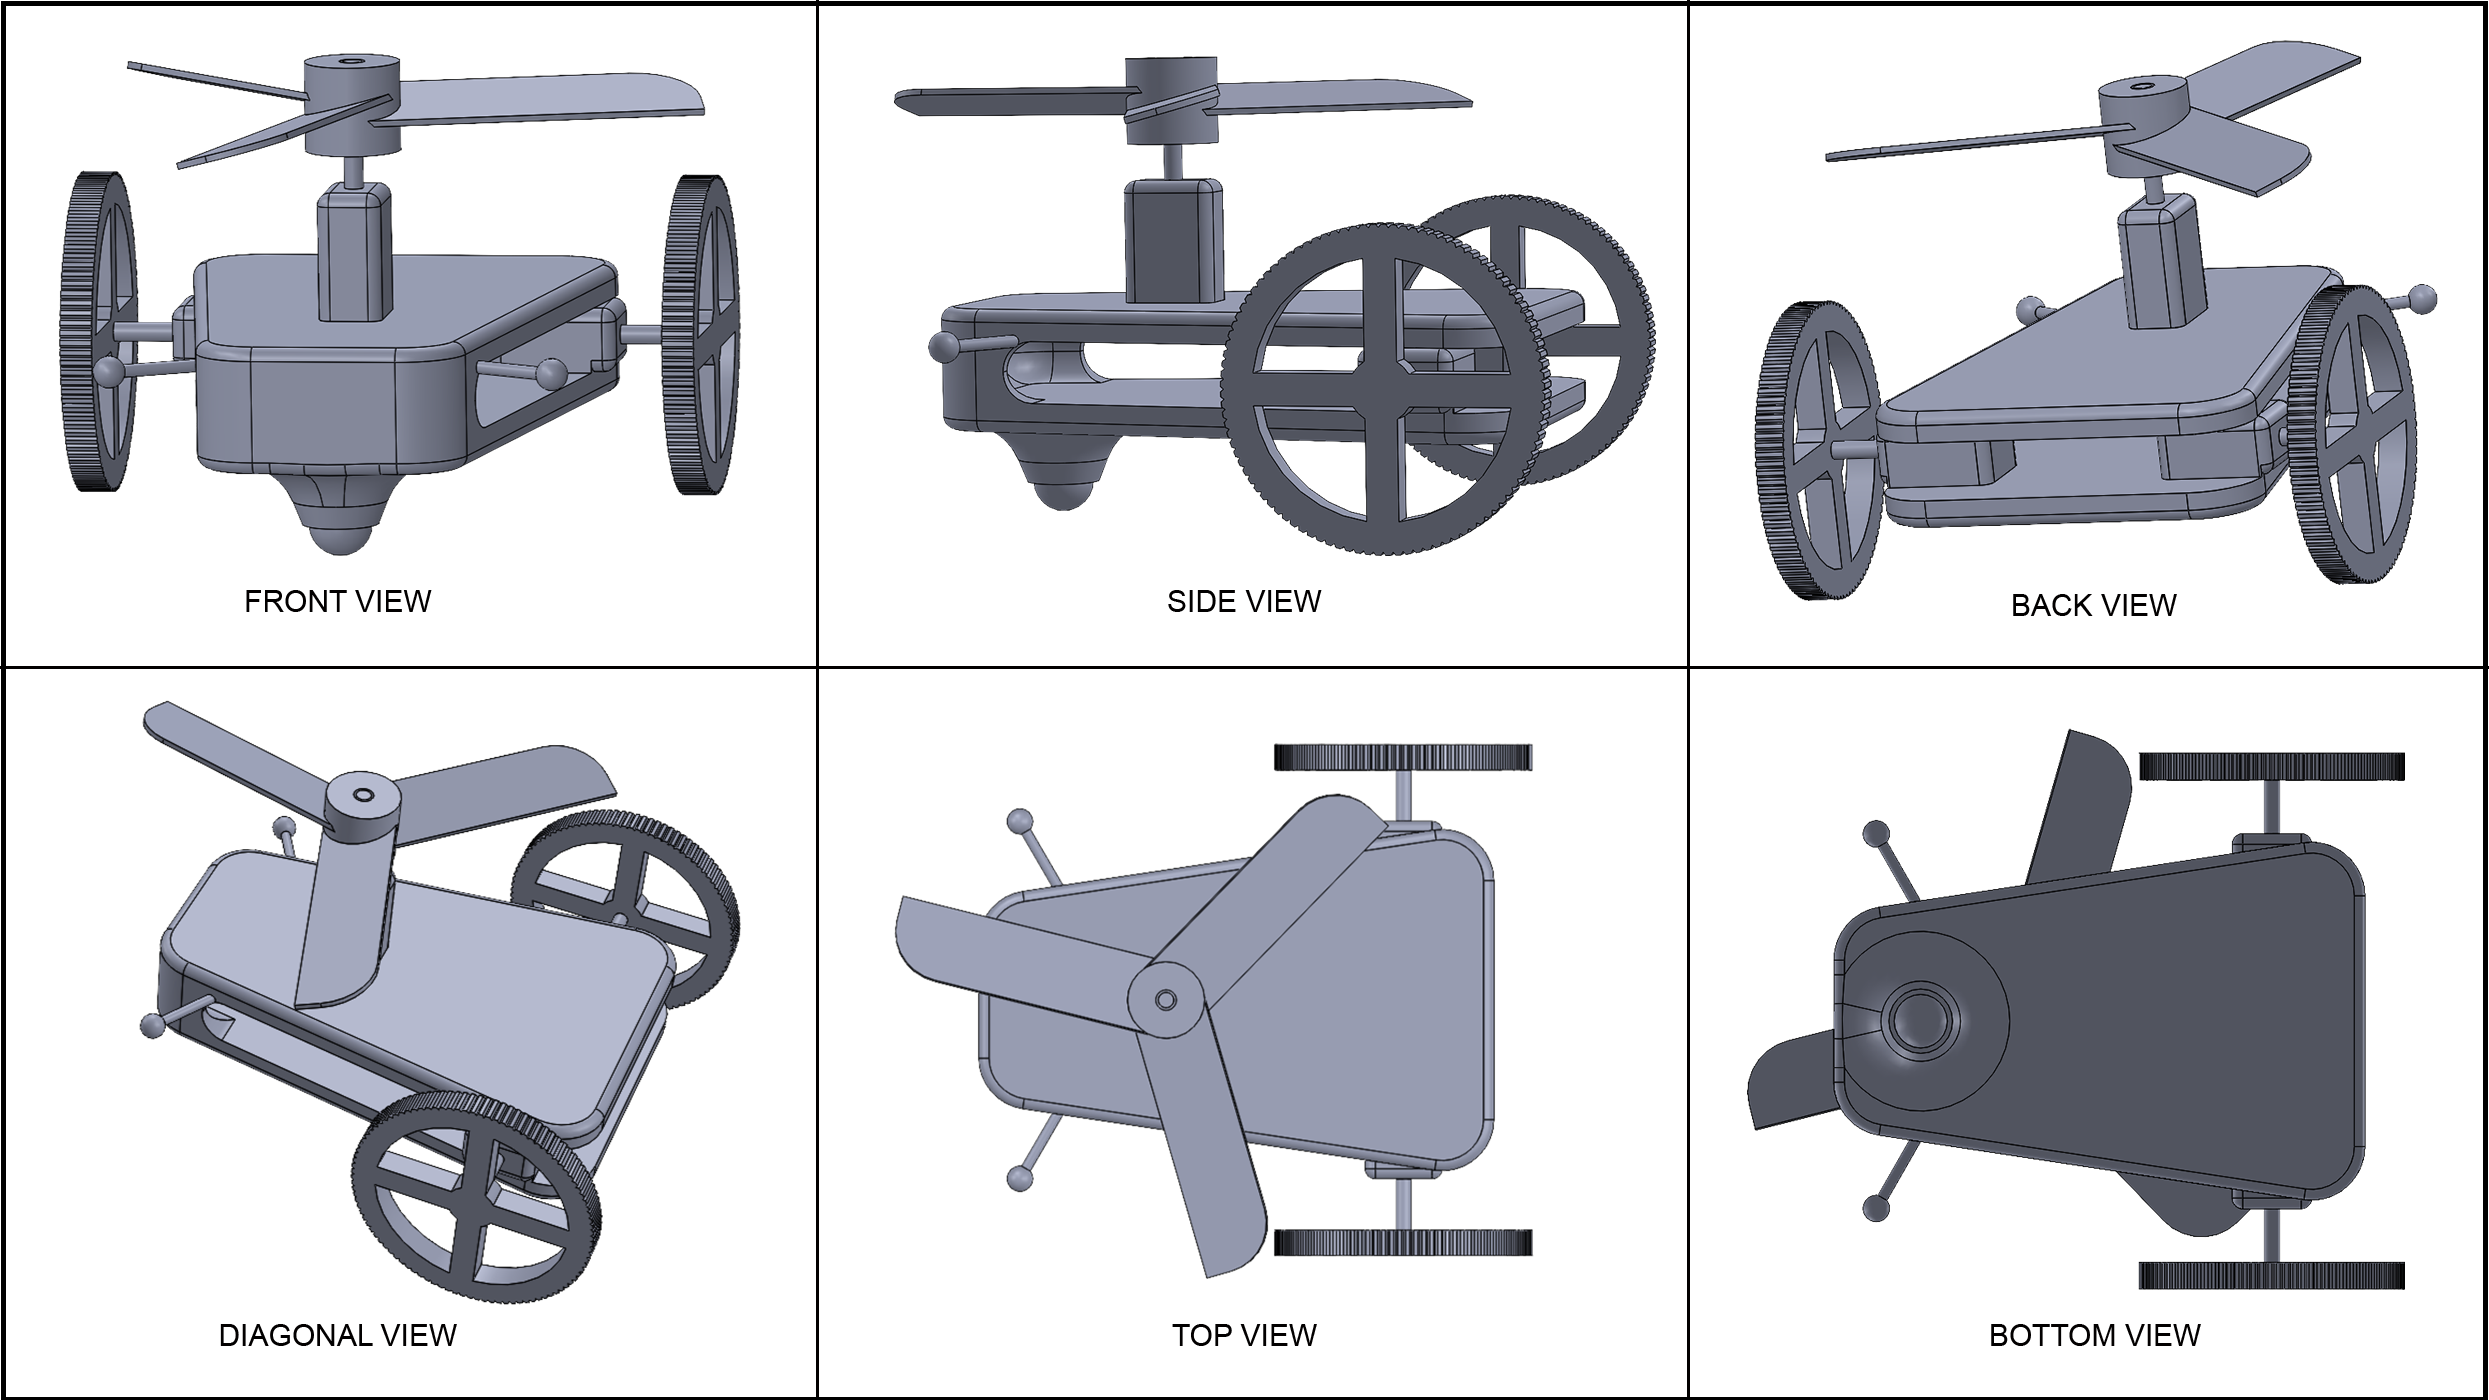
\includegraphics[width=13cm]{./images/vehicle_3D_grouped.png} 
            \caption{3D model of the proposed design}%
            \label{fig:3D_design}%
        \end{figure}

    So, finally, we are left with a vehicle which looks like Fig \ref{fig:3D_design}.
    \vspace{3mm}

    \subsection{Robot Configurations}
    \begin{itemize}
        \item \textbf{Sensors:} 2 sensors are attached on two sides of the vehicle for detecting the stimulus.
        \item \textbf{Actuators:} 2 wheels on two sides and 1 propeller on top for taking off the ground.
    \end{itemize}
\end{document}
